\documentclass{TIJMUjiaoanLL}
\pagestyle{empty}


\begin{document}


%课程名称
\kecheng{Linux系统概论}
%课程内容
\neirong{文件系统\ /\ 第4章}
%教师姓名
\jiaoshi{伊现富}
%职称
\zhicheng{讲师}
%教学日期(格式:XXXX年XX月XX日XX时-XX时)
\riqi{2018年5月21日10:00-12:00}
%授课对象(格式:XXX系XXXX年级XX班(硕/本/专科))
\duixiang{生物医学工程与技术学院2016级生信班(本)}
%听课人数
\renshu{28}
%授课方式
\fangshi{理论讲授}
%学时数
\xueshi{2}
%教材版本
\jiaocai{Unix入门经典,第1版}


%教案首页
\firstHeader
\maketitle
\thispagestyle{empty}

\mudi{
\begin{itemize}
  \item 掌握绝对路径和相对路径的表示方法,文件系统导航的基础命令及其常用参数,硬链接和软链接的区别,文件和目录的权限,权限的符号模式和绝对模式,修改权限的方法。
  \item 熟悉Linux的目录结构,Linux系统中的基本目录。
  \item 了解Linux中的各种文件类型,挂载文件系统的方法。
  \item 自学文件系统导航的其他命令及其参数。
\end{itemize}
}

\fenpei{
\begin{itemize}
  \item (5')引言与导入:介绍三种不同类型的文件系统。
  \item (20')文件系统基础:概述文件系统和分区的关系,介绍Linux的目录结构,讲解Linux系统的基本目录,比较绝对路径和相对路径。
  \item (25')文件系统导航:介绍文件和目录操作、管理的基础命令,详细讲解并演示cd、ls等重要的命令及其参数。
  \item (20')文件类型:介绍Linux系统中的常见文件类型,讲解链接的概念,比较硬链接和软链接的区别。
  \item (20')文件和目录权限:介绍文件和目录的权限,讲解权限的符号模式和绝对模式,演示并比较修改权限的方法。
  \item (5')挂载文件系统:介绍挂载和卸载文件系统的命令及其用法。
  \item (5')总结与答疑:总结授课内容中的知识点与技能,解答学生疑问。
\end{itemize}
}

\zhongdian{
\begin{itemize}
  \item 重点:绝对路径和相对路径的表示方法,权限的符号模式和绝对模式及其使用方法。
  \item 难点:硬链接和软链接的区别,权限的符号模式和绝对模式及其使用方法。
  \item 解决策略:通过实例讲解与操作演示帮助学生理解、记忆。
\end{itemize}
}

\waiyu{
  \vspace*{-10pt}
  \begin{multicols}{3}
    {\footnotesize
    文件系统(File System)

    绝对路径(Absolute Path)

    相对路径(Relative Path)

    主目录(Home Directory)

    根目录(Root Directory)

    \ 

    硬链接(Hard Link)

    软链接(Soft Link)
    
    符号链接(Symbolic Link)
    }
  \end{multicols}
  \vspace*{-10pt}
}

\fuzhu{
\begin{itemize}
  \item 多媒体:Linux的目录结构,Linux系统的基本目录。
  \item 板书:绝对路径和相对路径的表示方法,权限的符号模式和绝对模式及其使用方法。
  \item 演示:文件系统管理的基础命令,硬链接和软链接的区别。
\end{itemize}
}

\sikao{
  \vspace*{-10pt}
  \begin{multicols}{2}
  \begin{itemize}
    \item 列举Linux中的基本目录并解释其功能。
    \item 举例说明绝对路径和相对路径的区别。
    \item 列举几个进行文件系统导航的命令。
    \item 解释ls -l输出结果中每一列的含义。
    \item 比较Linux中的硬链接和软链接。
    \item Linux中的权限包括几种,针对哪些用户?
    \item 文件和目录的rwx权限有何异同?
    %\item 举例说明如何使用符号模式修改权限?
    %\item 举例说明如何使用绝对模式修改权限?
    \item 如何使用符号模式和绝对模式修改权限?
  \end{itemize}
  \end{multicols}
  \vspace*{-10pt}
}

\cankao{
\begin{itemize}
  %\item (美)Paul Love,Joe Merlino\ 等著,张楚雄,许文昭\ 译。Unix入门经典,清华大学出版社,2006。
  \item (美)Harley Hahn\ 著,张杰良\ 译。Unix \& Linux大学教程,清华大学出版社,2010。
  \item 鸟哥\ 著,王世江\ 改编。鸟哥的Linux私房菜——基础学习篇(第三版),人民邮电出版社,2010。
  \item 维基百科等网络资源。
\end{itemize}
}

\firstTail


%教案续页
\newpage
\otherHeader

\begin{enumerate}
  \item 引言与导入(5分钟)
    \begin{enumerate}
      \item 文件系统
	\begin{itemize}
	  \item 用户$\Leftrightarrow$操作系统$\Leftrightarrow$计算机
	  \item 用户$\Leftrightarrow$文件系统$\Leftrightarrow$硬盘
	\end{itemize}
      \item 文件系统的类型 \textcolor{red}{(由U盘格式化、FAT32/NTFS与单文件最大4G引出)}
	\begin{itemize}
\parpic[fr]{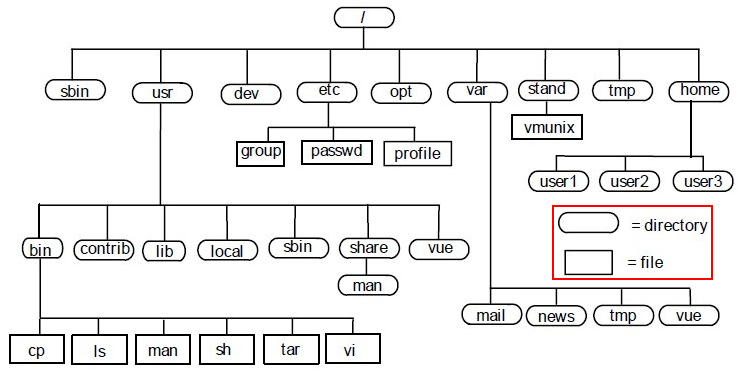
\includegraphics[width=9cm]{c3.filesystem.11.png}}
	  \item 面向磁盘的文件系统(本地):FAT,NTFS,EXT4,Btrfs,XFS,ISO9660
	  \item 面向网络的文件系统(网络):NFS,Samba
	  \item 专用或虚拟的文件系统:TMPFS,PROCFS
	\end{itemize}
    \end{enumerate}


  \item 文件系统基础(20分钟)
    \begin{enumerate}
      \item 文件系统和分区\\
      \textcolor{red}{(类比Windows:一块硬盘$\Rightarrow$C/D/E多个分区)$\Rightarrow$FAT32/NTFS不同文件系统}
	\begin{itemize}
	  \item 分区是信息的容器,包含整个硬盘或硬盘的一部分
          \item 文件系统是多个文件的逻辑集合,位于分区或磁盘上
          \item 一个分区通常只包含一个文件系统
	\end{itemize}
      \item Linux的目录结构
        \begin{itemize}
\parpic[fr]{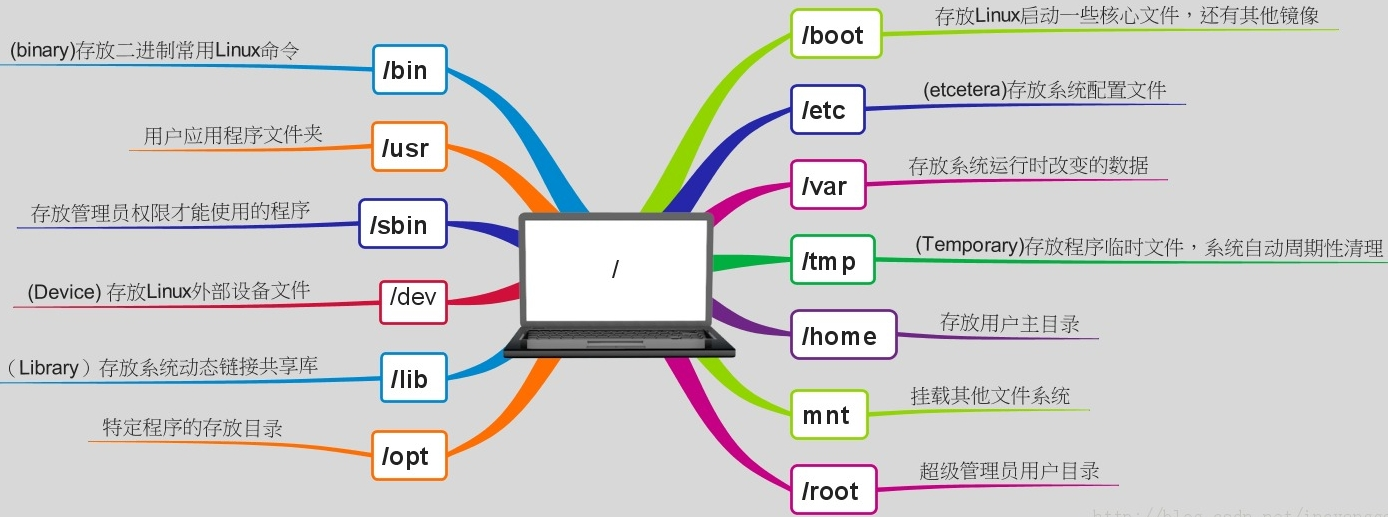
\includegraphics[width=11cm]{c3.filesystem.01.jpg}}
          \item Everything is a file.
          \item 自顶而下
          \item \textcolor{red}{一切源于根目录(/)}
          \item 分层结构
          \item \textcolor{red}{区分大小写}
        \end{itemize}
      \item Linux的基本目录
      \item \textcolor{red}{\textbf{【重点】}}路径\\
	\textcolor{red}{(类比:现实生活中的定位方式;比较:绝对路径和相对路径)}
	\begin{itemize}
	  \item 绝对路径:精确定位
	  \item 相对路径:相对于当前位置的定位
	    \vspace*{-10pt}
            \begin{multicols}{2}
	    \begin{itemize}
              \item \verb|.|:当前目录
              \item \verb|..|:上一层目录
              \item \verb|~|:当前用户的家目录
              \item \verb|-|:上一个工作目录
	    \end{itemize}
            \end{multicols}{}
	    \vspace*{-10pt}
	  \item \textcolor{red}{实例演示}:/var/log/mail vs.  ../../var/log/mail; /var/log/mail vs. ./mail
	  \item 优缺点:绝对路径——精确 vs. 冗长;相对路径——(多数时候)简短 vs. 隐患
	\end{itemize}
    \end{enumerate}

  \item 文件系统导航(25分钟)
    \begin{enumerate}
      \item 常用命令\textcolor{red}{(学生总结常见的操作,老师给出对应的命令)}
	\begin{itemize}
\parpic[fr]{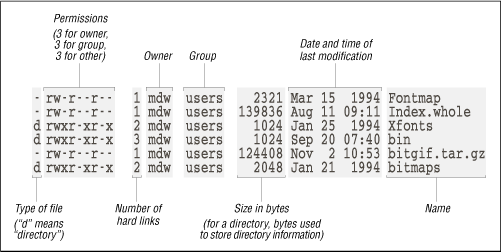
\includegraphics[width=9cm]{c3.ls.png}}
	  \item 目录导航:pwd,ls,cd,mkdir,rmdir,tree
	  \item 文件导航:file,cat,touch,cp,mv,rm,head,tail,more,less
	  \item 文件管理:which,whereis,find,df,du
	\end{itemize}
      \item 命令详解
	\begin{itemize}
	  \item ls:-a,-l\textcolor{red}{(通过实例讲解输出格式)}
	  \item rm:rmdir vs. rm,-f,-r
	  \item df,du:df -h,du -sh
	\end{itemize}
    \end{enumerate}

\otherTail
\newpage
\otherHeader

  \item 文件类型(20分钟)
    \begin{enumerate}
      \item 常见类型:-(普通文件),d(目录),l(符号链接),b,c,p,s
      \item inode\textcolor{red}{(类比:身份证号 vs. 姓名 vs. 曾用名/笔名/外号)}
        \vspace*{-10pt}
        \begin{multicols}{2}
          \begin{itemize}
	    \item 每一个文件都有一个inode
	    \item 使用inode而非文件名引用文件
	    \item 分区内inode是唯一的
	    \item 不同分区可以有相同的inode
	  \end{itemize}
        \end{multicols}
        \vspace*{-20pt}
        \begin{figure}[h]
	  \centering
	  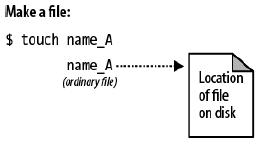
\includegraphics[width=4.8cm]{c3.ln1.png}
	  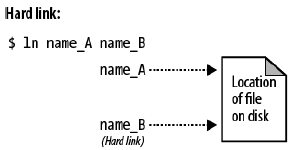
\includegraphics[width=5.2cm]{c3.ln2.png}
	  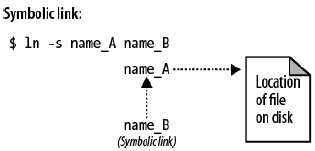
\includegraphics[width=5.6cm]{c3.ln3.png}
	\end{figure}
        \vspace*{-15pt}
      \item \textcolor{red}{\textbf{【难点】}}链接\textcolor{red}{(比较并进行实例演示)}
        \vspace*{-10pt}
        \begin{multicols}{2}
 	  \begin{itemize}
	    \item 硬链接:
	      \begin{itemize}
                \item 语法:ln source hardlink
		\item 本质:与原文件没有区别
		\item inode:与原文件相同
		\item 类比:不占空间的复制+同步更新
		\item 文件系统:不能跨越
		\item 修改链接:原文件随之变化
		\item 删除链接:原文件不受影响
		\item 删除原文件:链接不受影响
		\item 使用对象:只能是文件,目录无效
	      \end{itemize}
	    \item 软链接(符号链接):
	      \begin{itemize}
                \item 语法:ln -s source softlink
		\item 本质:保存原文件的路径
		\item inode:与原文件不同,是唯一的
		\item 类比:快捷方式
		\item 文件系统:能跨越
		\item 修改链接:原文件随之变化
		\item 删除链接:原文件不受影响
		\item 删除原文件:链接失效
		\item 使用对象:文件和目录
	      \end{itemize}
	  \end{itemize}
        \end{multicols}
        \vspace*{-10pt}
    \end{enumerate}

  \item 文件和目录权限(20分钟)
    \begin{enumerate}
      \item 权限简介\textcolor{red}{(比较文件和目录的异同)}
	\vspace*{-10pt}
	\begin{figure}[h]
	  \centering
%\parpic[fr]{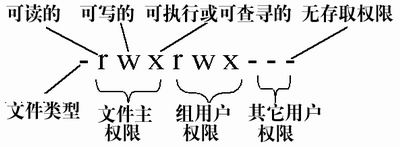
\includegraphics[width=5cm]{c3.ugo.01.png}}
          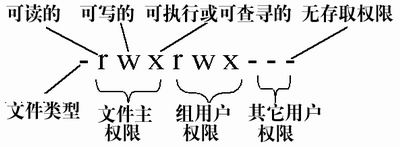
\includegraphics[width=7cm]{c3.ugo.01.png}
	  \quad
          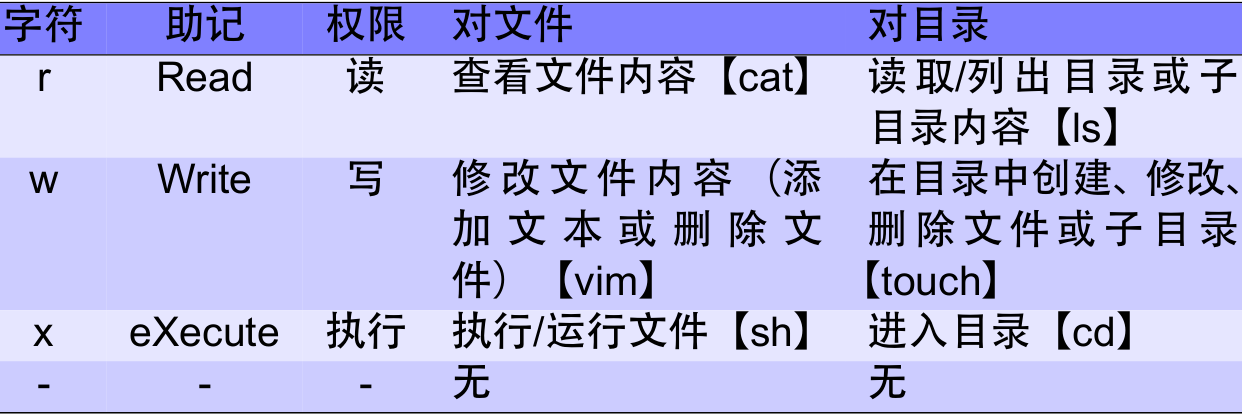
\includegraphics[width=8cm]{c3.rwx.png}
	\end{figure}
	\vspace*{-10pt}
      \item \textcolor{red}{\textbf{【重点、难点】}}修改权限\textcolor{red}{(实例讲解,操作演示)}
	\begin{itemize}
	  \item 符号模式:容易理解
            \vspace*{-10pt}
            \begin{multicols}{3}
	      \begin{itemize}
		\item 用户:
		  \begin{itemize}
		    \item u:User,用户
		    \item g:Group,组
		    \item o:Other,其他人
		    \item a:All,所有人
		  \end{itemize}
		\item 操作:
		  \begin{itemize}
		    \item +:添加
		    \item -:删除
		    \item =:指定

		    \ 
		  \end{itemize}
		\item 权限:
		  \begin{itemize}
		    \item r:Read,读
		    \item w:Write,写
		    \item x:eXecute,执行
		    %\item -:无
		  \end{itemize}
	      \end{itemize}
            \end{multicols}
            \vspace*{-10pt}
	  \item 绝对模式:更加高效
            \vspace*{-10pt}
            \begin{multicols}{2}
	      \begin{itemize}
		\begin{minipage}[t]{0.3\textwidth}
		\item 基本权限:
		  \begin{itemize}
		    \item 0:-\ -\ -,无权限
		    \item 1:-\ -x,可执行
		    \item 2:-w-,可写
		    \item 4:r-\ -,可读
		  \end{itemize}
		\end{minipage}
		\begin{minipage}[t]{0.8\textwidth}
		\item 引申权限:
		  \begin{itemize}
		    \item 3(=1+2):-wx,可写、可执行
		    \item 5(=1+4):r-x,可读、可执行
		    \item 6(=2+4):rw-,可读、可写
		    \item 7(=1+2+4):rwx,可读、可写、可执行
		  \end{itemize}
		\end{minipage}
	      \end{itemize}
            \end{multicols}
            \vspace*{-10pt}

	  \item \textcolor{red}{修改实例}
	    \begin{itemize}
	      \item 符号模式:chmod u-x file, chmod o+wx file, chmod g=r-x file
	      \item 绝对模式:chmod 740 file, chmode 755 file
	    \end{itemize}
	\end{itemize}
    \end{enumerate}

\otherTail
\newpage
\otherHeader

  \item 挂载文件系统(5分钟)
    \begin{enumerate}
      \item 语法
        \begin{itemize}
          \item 挂载:mount -t FILE.SYSTEM.TYPE DEVICE DIRECTORY
          \item 卸载:umount DEVICE.TO.UNMOUNT
        \end{itemize}
      \item 实例\textcolor{red}{(以光盘为例)}
        \begin{itemize}
          \item 挂载:mount -t iso9660 /dev/cdrom /mnt/cdrom
          \item 卸载:umount /dev/cdrom
        \end{itemize}
    \end{enumerate}

  \item 总结与答疑(5分钟)
    \begin{enumerate}
      \item 知识点
	\begin{itemize}
	  \item Linux的目录结构,基本目录,绝对路径和相对路径
	  \item Linux的常见文件类型,硬链接和软链接
	  \item Linux中文件和目录的权限,权限的符号模式和绝对模式
	  \item 文件系统导航的常见命令,挂载和卸载的命令
	\end{itemize}
      \item 技能:命令行操作
	\begin{itemize}
          \item 文件系统的导航
          \item 硬链接和软链接的创建
          \item 文件权限的修改
          \item 文件系统的挂载和卸载
	\end{itemize}
    \end{enumerate}

\end{enumerate}

\otherTail


\end{document}

